\section{实验}
\label{sec:exp}

本节依次检验第\ref{sec:method}节的三个选择：加算能否消除选边错误（第\ref{sec:compute}节）；最大后悔值能否找出高风险任务、梯度搜索是否高效（第\ref{sec:rank}、\ref{sec:budget}节）；判定粗图不可信后应如何行动（第\ref{sec:respond}节）。第\ref{sec:scope}节考察换海区与换地图时结论的适用范围。

\subsection{实验设置}
全部参数在开发年份（2019--2021年）标定，在测试年份（2022--2024年）只评价一次。主设置为黑潮区（测试任务623个）；为检验结论的适用范围，我们在湾流（33°--41°N、75°--67°W，643个）与阿古拉斯回流区（35°--43°S、14°--22°E，618个）重复了同一流程，并在黑潮区让航行器改带美国国家海洋和大气管理局的近实时融合卫星测高地转流图（0.25°，3天前，648个）；后两种设置的检验内容在获取数据之前即已确定。对比方法包括：同一张粗图上的粗、中、细网格求解（细网格求解即基线）；集合平均选边（32个集合成员）与选最大后悔值较小的一侧；四种就地测流；总是上浮取当天1°或0.5°图；以及本文的超阈值时上浮取图与超阈值时保守改选。与基线的配对差按天整组重抽样（2000次）求95\%置信区间，区间不含0时称差异显著。

\subsection{加算消除不了环境歧义}
\label{sec:compute}
在同一张粗图上增加计算，只能纠正很少一部分选边错误。在黑潮测试年份，从粗网格求解改为细网格求解，计算量增加64倍，改变了64个任务的选择，其中38个改对、26个改错，选错率仅从21.7\%降至19.7\%；换成当天0.5°图，选错率则降至10.4\%（图\ref{fig:ambiguity}(a)）。其余三种设置中，加算前后选错率的变化都不超过1个百分点。

\begin{figure}[t]
\centering
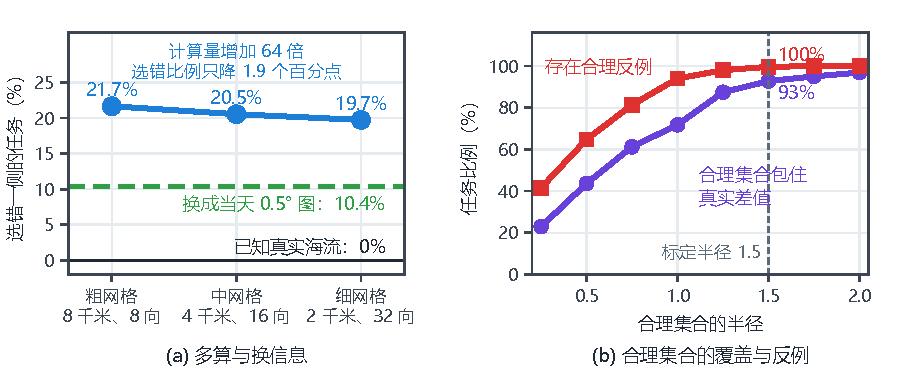
\includegraphics[width=0.92\linewidth]{fig_route_ambiguity}
\caption{求解计算量与环境信息对选边错误的不同作用（黑潮测试年份）。(a) 选错一侧的任务比例：粗网格、中网格、细网格求解依次为21.7\%、20.5\%、19.7\%，换成当天0.5°图降至10.4\%；(b) 随合理集合半径增大，合理集合包住真实左右航时差的任务比例（开发年份）与存在合理反例的任务比例（测试年份）。加算只能消除很少一部分错误；在足以包住真实海流的合理集合中，几乎每个决定都存在合理反例。}
\label{fig:ambiguity}
\end{figure}

加算无效的原因在于环境歧义普遍存在。在覆盖94\%真实左右航时差的标定半径下，黑潮99.7\%的测试任务都能找到合理反例（图\ref{fig:ambiguity}(b)），湾流与阿古拉斯回流区也分别为98.8\%与99.2\%。这些任务的粗图本身容许两种相反的选择，求解得再细也无法从中分辨；因此，“有没有合理反例”不足以区分任务，需要看反例会让当前选择多花多少时间。

\subsection{最大后悔值找得出额外航时所在}
\label{sec:rank}
按最大后悔值排序，能把大部分额外航时集中到少数任务上。黑潮测试年份的额外航时高度集中，额外航时最大的10\%任务占全部额外航时的92\%；按最大后悔值排在前20\%的任务占67\%，而按改变选边的成员比例排序只占49\%，按粗图左右航时差排序只占34\%（图\ref{fig:risk}(a)）。在湾流、阿古拉斯回流区与改带卫星测高地转流图时，最大后悔值排在前20\%的任务分别占71\%、53\%与67\%，均高于改变选边的成员比例（49\%、36\%与52\%）。

\begin{figure}[t]
\centering
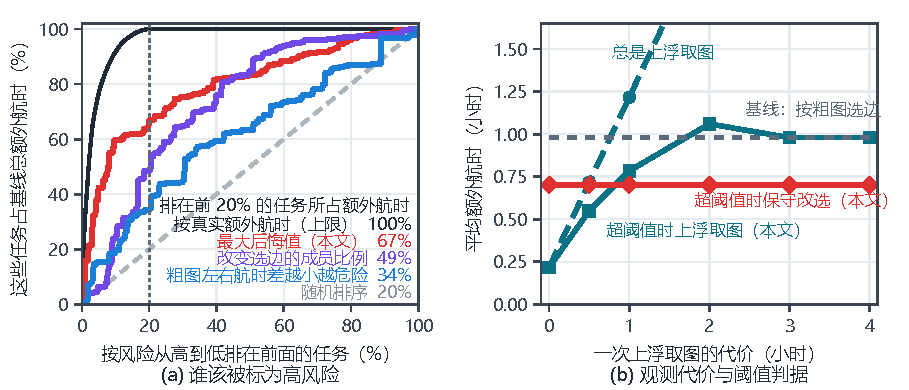
\includegraphics[width=0.92\linewidth]{fig_route_risk}
\caption{最大后悔值的风险排序与上浮代价（黑潮测试年份）。(a) 按不同指标从高到低排序时，排在前面的任务累计所占的额外航时；(b) 平均额外航时随单次上浮取当天0.5°图的代价的变化。最大后悔值把大部分额外航时集中到少数任务上；单次上浮代价低于约1小时时，超阈值时上浮取图最优。}
\label{fig:risk}
\end{figure}

这一优势来自度量的对象，而不是样本的多少。改变选边的成员比例只数有多少集合成员改选，把多花半小时与多花十几小时等同看待；最大后悔值则直接度量改选的代价。即使集合成员增至1024个，按改变选边的成员比例排在前20\%的任务也只占44\%，而在同一批成员上计算的后悔值的集合平均可达67\%（图\ref{fig:budget}(b)）。在黑潮主设置中，阈值判据（$\theta=8$小时）标记了47\%的任务，这些任务囊括了82\%的额外航时。

\subsection{梯度搜索以约二十九分之一的求解次数达到同样的选边效果}
\label{sec:budget}
在决定选哪一侧时，梯度搜索约71次航线求解，即达到集合平均选边使用1024个集合成员（2048次求解）的效果（图\ref{fig:budget}(a)）。选最大后悔值较小的一侧，等价于按合理集合给出的左右航时差范围的中点选边：若航时差随流场线性变化，这一中点就是粗图的航时差，二者选择相同；只有一侧的最不利情形比另一侧严重得多时，才会改选。

\begin{figure}[t]
\centering
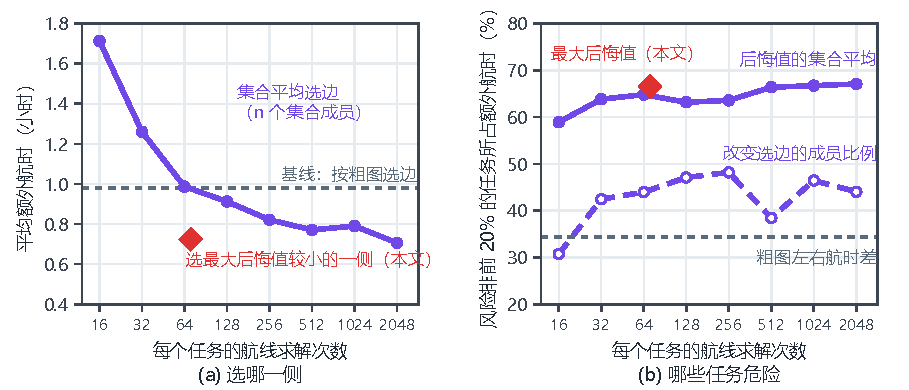
\includegraphics[width=0.92\linewidth]{fig_route_budget}
\caption{集合成员数量与梯度搜索的比较（黑潮测试年份）。(a) 平均额外航时随每个任务航线求解次数的变化：曲线为集合平均选边，菱形为梯度搜索后选最大后悔值较小的一侧；(b) 排在前20\%的任务所占的额外航时：曲线为在相同集合成员上计算的后悔值的集合平均与改变选边的成员比例，菱形为最大后悔值。选对一侧要上千个集合成员才能估准，梯度搜索约71次求解即可做到；排序的优劣则取决于是否度量多花的时间。}
\label{fig:budget}
\end{figure}

集合平均选边估计的是同一个修正量，却受抽样误差左右。32个集合成员时，集合平均的抽样误差（中位数2.4小时）大于它要估计的修正量（中位数1.7小时），改选多由噪声驱动，平均额外航时为0.99小时，显著高于梯度搜索后保守选边的0.72小时；集合成员增至数百个以上，二者才不再有显著差异。对算力有限的航行器而言，梯度搜索省下的正是这上千次航线求解。

\subsection{判定粗图不可信后，取新信息最划算}
\label{sec:respond}
对被阈值判据标记的任务，最划算的回应是获取新信息，在粗图误差大的海区尤其如此。湾流与阿古拉斯回流区的粗图误差大，基线的平均额外航时分别为3.56小时与6.87小时；即使每次上浮计1小时，超阈值时上浮取图仍使二者显著降至1.31小时与2.20小时（表\ref{tab:scope}）。在湾流，它只在约三分之二的任务上上浮，就优于总是上浮（1.53小时）；在阿古拉斯回流区，粗图误差普遍较大，总是上浮（1.98小时）略好于按阈值上浮。在黑潮主设置中，单次上浮代价低于约1小时时，超阈值时上浮取图是最优回应（图\ref{fig:risk}(b)）。

\begin{figure}[t]
\centering
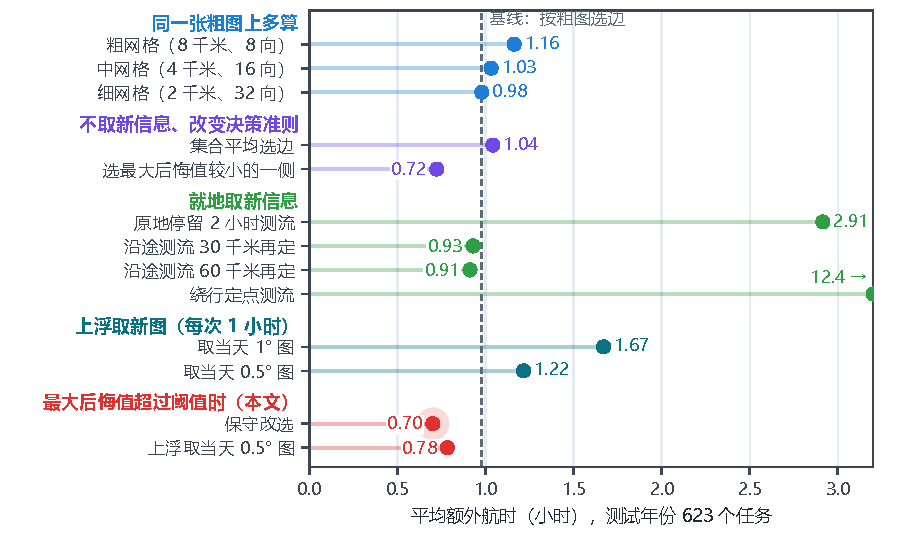
\includegraphics[width=0.88\linewidth]{fig_route_main}
\caption{黑潮测试年份623个任务上各类行动的平均额外航时（虚线为基线0.98小时，数值标在点旁）。由上至下依次为：同一张粗图上多算、不取新信息而改变选边准则、就地测流、总是上浮取图、最大后悔值超过阈值时的两种回应。加算与就地测流均未显著改善，超阈值时保守改选显著降低了额外航时。}
\label{fig:main}
\end{figure}

就地测流视野有限，多数情况下得不偿失（图\ref{fig:main}）。原地停留测流花2小时只测到起点一处；绕行定点测流平均要先花15.4小时赶到测点；沿途测流30千米很少改变判断（只有3.4\%的任务换边），测完60千米再换边又已走过半程。只有在额外航时很大的阿古拉斯回流区，沿途测流30千米才显著降低了额外航时，但仍不如上浮取图。

不能观测时，改选最大后悔值较小的一侧同样能降低额外航时。黑潮主设置中，超阈值时保守改选使平均额外航时从0.98小时降至0.70小时（配对差$-0.28$小时，95\%置信区间$[-0.51, -0.07]$）。它改选的41个任务中，23个改对、平均各省10.1小时，18个改错、平均各多花3.3小时：被避开的一侧往往有很大的下行风险，改对的收益远大于改错的代价。

\subsection{适用范围}
\label{sec:scope}
前两项发现在四种主要设置中都成立（第\ref{sec:compute}、\ref{sec:rank}节），回应的收益则取决于粗图误差的大小与结构（表\ref{tab:scope}）。粗图越可信，检验越少干预：航行器直接携带当天0.5°图时，基线的平均额外航时只有0.17小时，两种超阈值回应几乎不改变选边；航速降至0.75米/秒时，选错的代价增大，超阈值时上浮取图把额外航时从2.43小时降至1.32小时。用历史相似日的小尺度差代替标定的误差模型构造合理集合时，超阈值时保守改选（0.95小时）与基线（0.99小时）无显著差异，说明合理集合必须由真实的误差结构标定。

\begin{table}[tb]
\centering
\caption{各设置下的测试年份结果（额外航时单位：小时；上浮指取当天0.5°图）。}
\label{tab:scope}
\small
\begin{tabular}{@{}p{0.19\linewidth}>{\centering\arraybackslash}p{0.088\linewidth}>{\centering\arraybackslash}p{0.088\linewidth}>{\centering\arraybackslash}p{0.088\linewidth}>{\centering\arraybackslash}p{0.088\linewidth}>{\centering\arraybackslash}p{0.088\linewidth}>{\centering\arraybackslash}p{0.088\linewidth}>{\centering\arraybackslash}p{0.088\linewidth}@{}}
\toprule
设置 & 测试任务 & 存在合理反例 & 基线选错率 & 基线额外航时 & 超阈值时保守改选 & 超阈值时上浮取图 & 最大后悔值前20\%所占额外航时 \\
\midrule
黑潮主设置 & 623 & 99.7\% & 19.7\% & 0.98 & 0.70 & 0.78 & 67\% \\
粗图换成当天0.5°图 & 349 & 64.5\% & 8.0\% & 0.17 & 0.17 & 0.16 & 60\% \\
航速降至0.75米/秒 & 347 & 99.1\% & 18.4\% & 2.43 & 1.80 & 1.32 & 74\% \\
消融：合理集合改用相似日差值 & 349 & 99.4\% & 19.5\% & 0.99 & 0.95 & 0.77 & 64\% \\
湾流 & 643 & 98.8\% & 19.4\% & 3.56 & 4.00 & 1.31 & 71\% \\
阿古拉斯回流区 & 618 & 99.2\% & 27.7\% & 6.87 & 6.49 & 2.20 & 53\% \\
改带卫星测高地转流图 & 648 & 81.0\% & 19.6\% & 0.79 & 0.71 & 0.64 & 67\% \\
\bottomrule
\end{tabular}

\end{table}

不观测时的保守改选只适用于两侧最坏情形差别分明的海区。湾流与阿古拉斯回流区分别有8.7\%与16.2\%的任务在真实海流中有一侧无法通行（黑潮为1.0\%）；这类任务的合理集合中既有堵死左侧、也有堵死右侧的流场，两侧最大后悔值都接近上限，选较小的一侧近于随机，因此超阈值时保守改选在两海区均无显著收益。若只在两侧最大后悔值之差超过数值误差容限时才改选，这种近于随机的改选即可避免（湾流3.45小时，阿古拉斯回流区6.72小时，均与基线无显著差异）；在这两个海区，被标记的任务应交给上浮取图。

改带真实卫星测高地转流图时，加算无效与最大后悔值排序两项发现仍然成立（选错率从19.9\%变为19.6\%；前20\%的任务占67\%的额外航时），但各种回应均未显著降低额外航时，存在合理反例的任务也降至81.0\%。即使换成当天的测高图，选错率仍为18.5\%，而当天0.5°模式图只有8.6\%，说明测高图与再分析场之间的差异主要是两种产品的系统差，不随时效消失。

本研究仍有局限：单次任务中的海流视为定常；真实海流取自再分析场，平滑了亚中尺度过程；只考虑单个禁航区的左右选边；并假设选定一侧后航行器按真实海流以最优轨迹航行。
